\chapter{Design}
\label{chap:design}

\section{Overall Design}
\label{sec:overall_design}
The system's design can be broken down into three core areas: the physical mechanical structure, the electronic hardware architecture, and the software architecture. This chapter details the design decisions made in each of these areas. Figure \ref{fig:golfbot_system_diagram} provides a visual overview of the completed robot.

\begin{figure}[h!]
    \centering
    \includegraphics[width=0.7\linewidth]{figures/complete.png}
    \caption{GolfBot System Diagram}
    \label{fig:golfbot_system_diagram}
\end{figure}

\section{Mechanical Design}
\label{sec:mechanical_design}
The mechanical design focuses on the robot's physical construction, ensuring stability, and the proper placement of all sensors and actuators.

\subsection{Chassis and Drivetrain}
\label{ssec:chassis_drivetrain}
The robot's structure is based on a lightweight aluminum chassis with main body dimensions of 500 mm x 360 mm x 115 mm. It uses a differential drive architecture, powered by two wheel hub motors with a wheel diameter of 165 mm and a distance between the motors of 570 mm. For stability, the drivetrain is supported by rubber caster wheels.

The motor hubs and casters are mounted on two swing arms, which function as a simple suspension system. This allows the robot's main body to remain relatively horizontal while the swing arms absorb minor bumps from uneven terrain. The wheels provide a ground clearance of 100 mm, sufficient for overcoming common obstacles on a golf course fairway. To protect the electronics, all internal components are housed within the main body frame, secured in custom 3D-printed holders and attached with strong, double-sided Velcro to prevent movement during operation.

\subsection{Component Mounting}
\label{ssec:component_mounting}
To ensure optimal data collection, custom mounts were designed for the primary sensors. An L-shaped 25 mm aluminum box section is mounted on top of the robot's aluminum plate. This structure holds the camera 300 mm in front of the robot and 600 mm above the ground, providing a clear and effective field of view. To protect the camera from direct sunlight and physical impacts, it is housed in a 3D-printed holder featuring a 90-degree hinge, which ensures the camera is positioned orthogonally to the ground.

The same aluminum arm also supports a 2 mm thick stainless steel circular plate that serves as a ground plane for the RTK-GPS rover antenna. Additionally, a stand for the LCD screen, used for the graphical user interface, is mounted on the top of the aluminum plate.

\subsection{Dispensing and Repair Mechanism}
\label{ssec:dispenser_mechanism}
The repair system is mounted at the rear of the robot. A laser-cuted and folded stainless steel bracket holds the sand dispenser 100 mm above the ground and approximately 900 mm behind the camera's center point. The dispenser itself is 3D-printed from \gls{PLA}. Its core is a screw auger mechanism, powered by a NEMA 17 stepper motor, which pushes the sand-seed mixture from a hopper out through a nozzle.

Mounted directly behind the dispenser nozzle is a rubber-mounted brush. This brush extends 60 mm from the nozzle and serves to evenly spread the dispensed material, ensuring the divot is filled smoothly. It is attached to the same stainless steel bracket using custom 3D-printed mounts.

\subsection{RTK Base Station Design}
\label{ssec:rtk_base_design}
The ArduSimple RTK system necessitates a stationary base station to deliver correction data to the rover. To achieve this, the base module is securely enclosed within a waterproof plastic box, as shown in Figure~\ref{fig:base_box}, and mounted on a metal pipe. A circular, laser-cut metal plate is affixed to the top of the pipe to support the RTK base antenna. This entire setup is designed to remain stationary, ensuring signal integrity by positioning it at the highest point within the robot's operational area. The base station is powered through a standard \gls{USB} cable, which can be connected to a laptop or a simple USB wall adapter. As shown in Figure~\ref{fig:base_antenna}, the base antenna setup is depicted here.

\begin{figure}[H]
    \centering
    \begin{subfigure}{0.35\linewidth}
        \centering
        \includegraphics[height=0.35\textheight]{figures/base_box.png}
        \caption{RTK Base Box}
        \label{fig:base_box}
    \end{subfigure}
    \begin{subfigure}{0.35\linewidth}
        \centering
        \includegraphics[height=0.35\textheight]{figures/base_antenna.png}
        \caption{RTK Base Antenna Setup}
        \label{fig:base_antenna}
    \end{subfigure}
\end{figure}

\section{Hardware Architecture}
\label{sec:hardware_architecture}
The hardware architecture of the GolfBot is designed as a centralized system, with the Seeed reComputer J4102 (carrying the NVIDIA Jetson Orin Nano module) serving as the primary processing unit or "brain." This central controller is responsible for running the high-level software, including the AI model, navigation logic, and the ROS 2 framework. All other electronic components are connected to this central hub, creating a clear data and power distribution network.

The overall electronic layout and data pathways are illustrated in Figure \ref{fig:hardware_diagram}. The primary communication interface is USB, which provides a robust and standardized way to connect most of the high-bandwidth sensors and controllers.

\begin{figure}[h!]
    \centering
    % The user will create and add this figure
    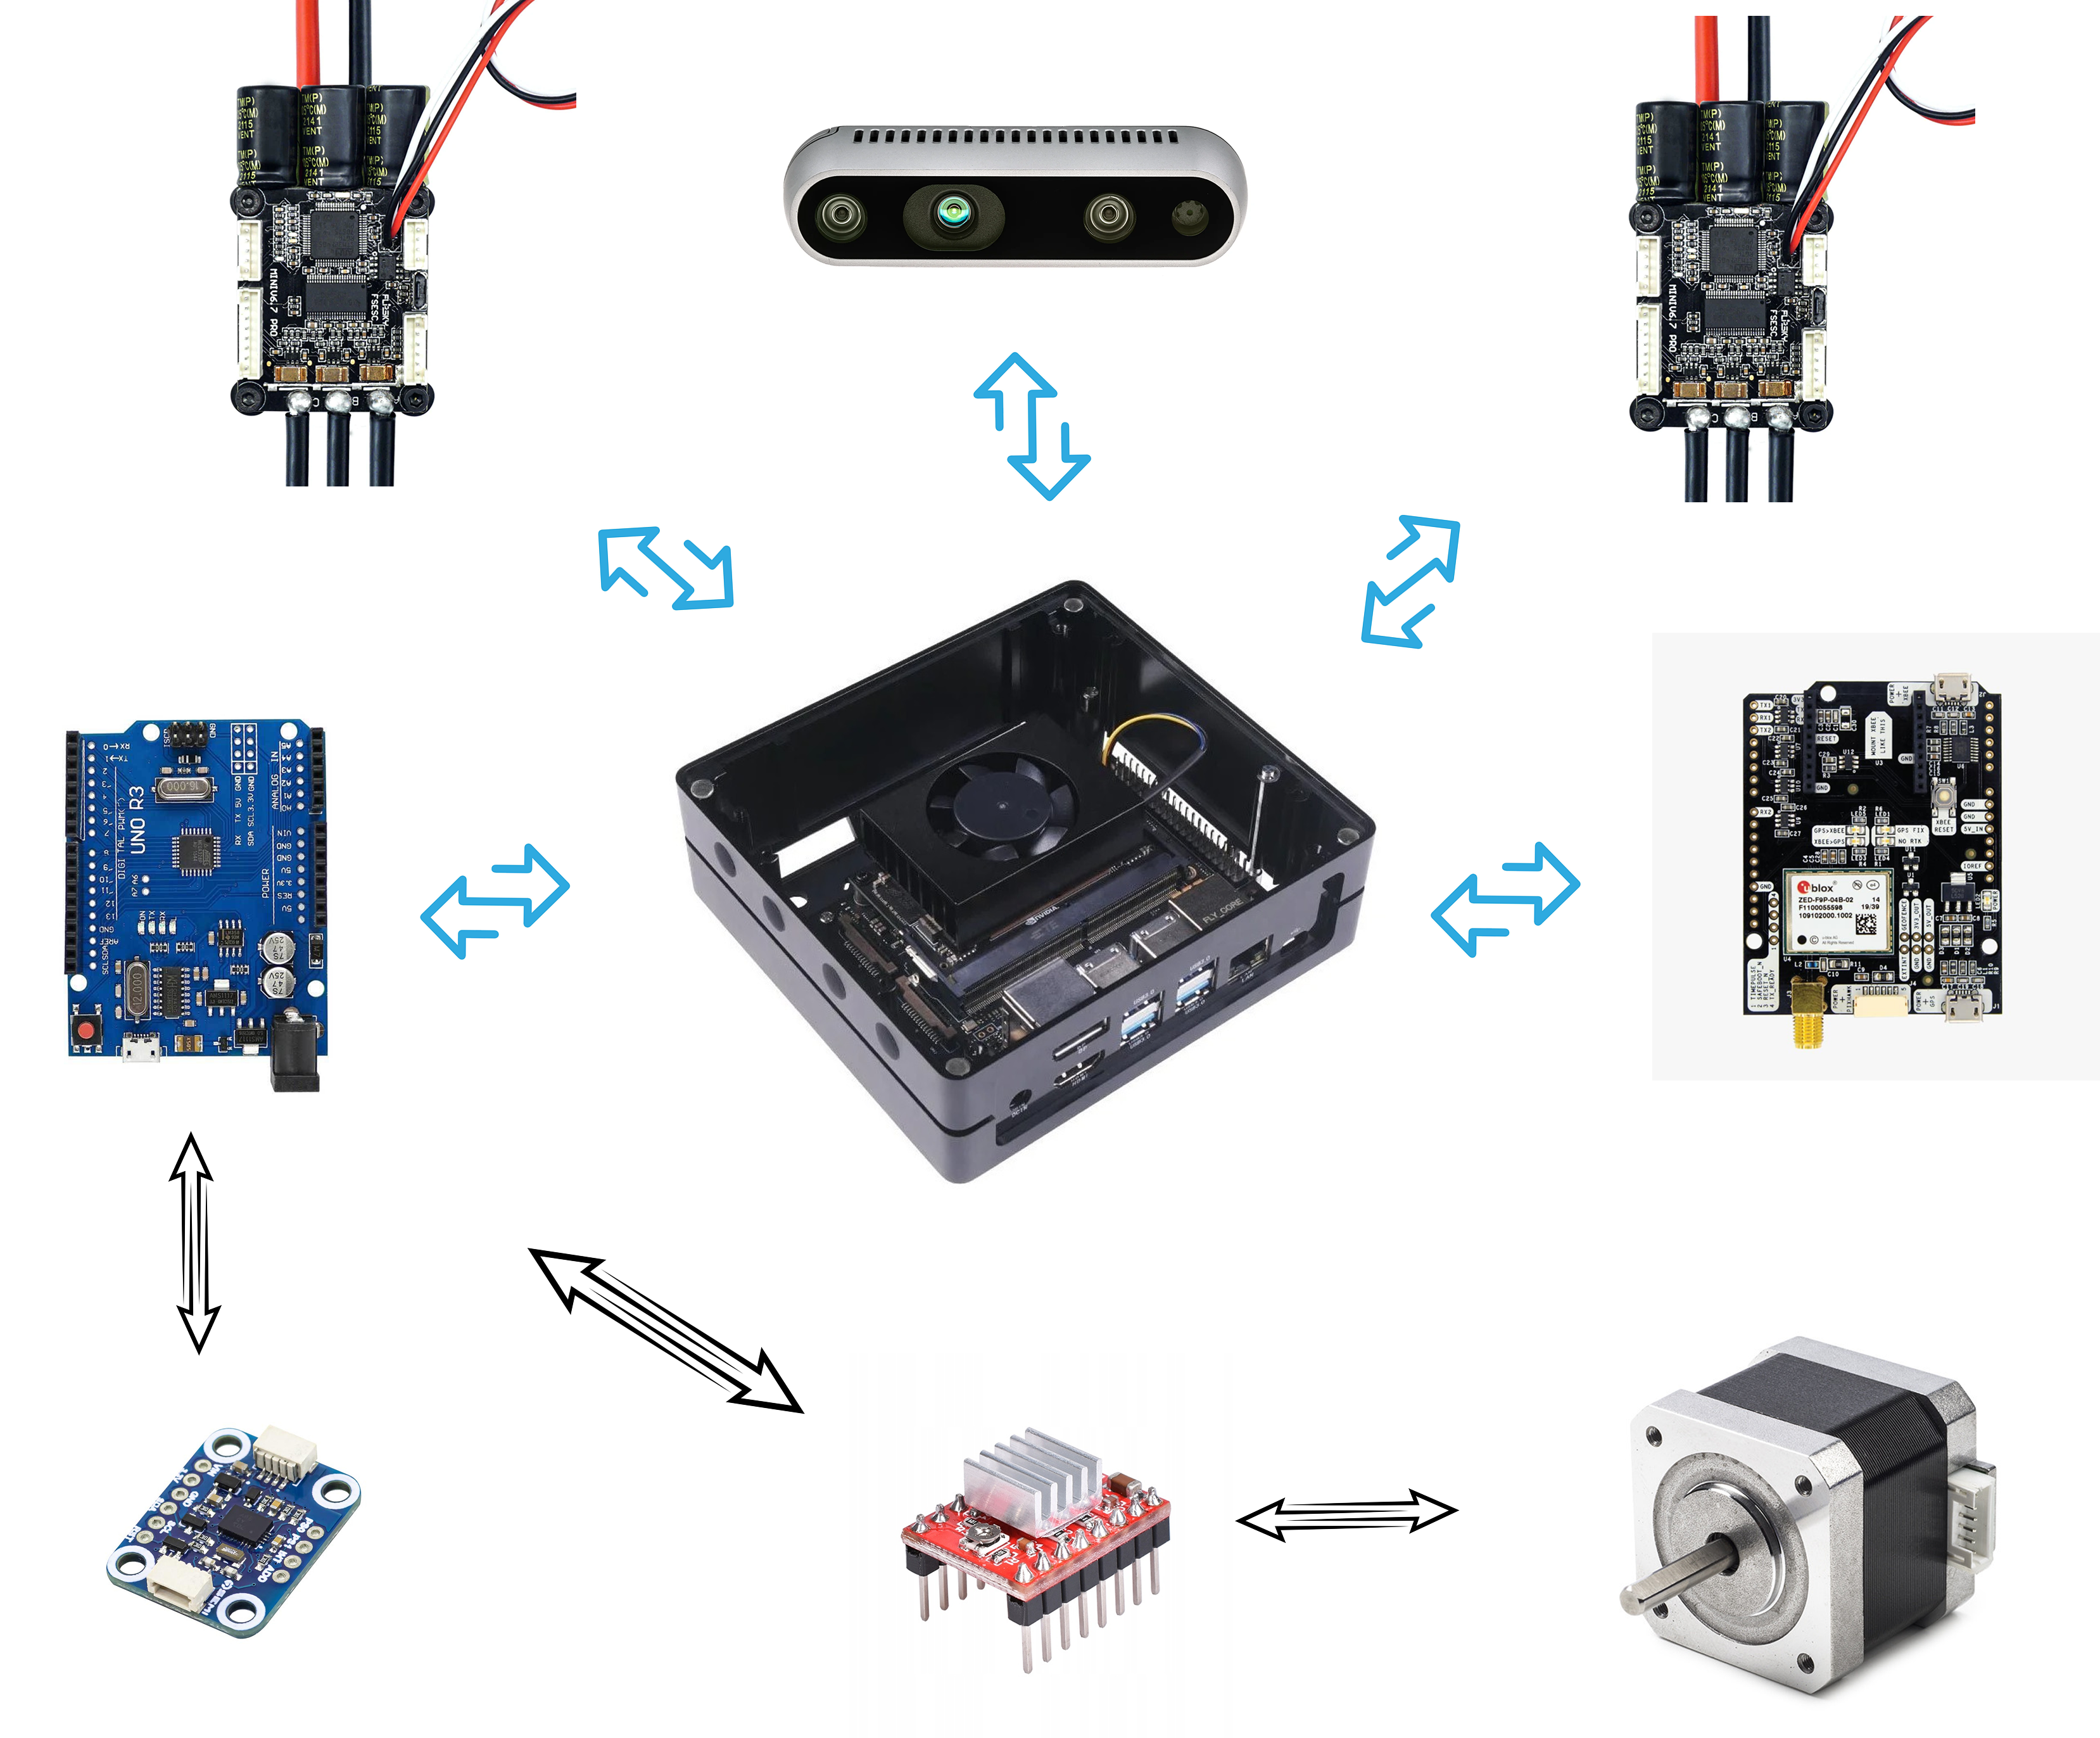
\includegraphics[width=1\linewidth]{figures/hardware_diagram.png}
    \caption{The centralized hardware architecture of the GolfBot, showing the primary data connections to the Jetson Orin controller.}
    \label{fig:hardware_diagram}
\end{figure}

\subsection{Component Connectivity}
The electronic components are organized around the Jetson controller as follows:
\begin{description}
    \item[Drivetrain Controllers] The two VESC motor controllers, one for each drive wheel, are connected to the Jetson via USB. They receive high-level velocity commands from the main controller and are responsible for the precise, low-level control of the brushless DC motors.
    \item[Vision System] The Intel RealSense D435i camera, the robot's primary sensor, is connected directly to a high-speed USB 3.0 port on the Jetson to ensure sufficient bandwidth for streaming both color and depth data.
    \item[Localization System] The ArduSimple simpleRTK2B RTK-GPS module is connected via USB. It streams positioning data to the Jetson, which is used for global navigation.
    \item[Low-Level Microcontroller Bridge] An Arduino Uno acts as a dedicated sub-controller for real-time tasks. It is connected to the Jetson via a single USB port and manages a group of its own peripherals:
    \begin{itemize}
        \item The \textbf{BNO055 IMU sensor} is connected to the Arduino, which reads the orientation data.
        \item The \textbf{A4988 stepper motor driver} receives step and direction signals from the Arduino to control the \textbf{NEMA 17 stepper motor} for the dispensing mechanism.
    \end{itemize}
    This design offloads the hard real-time motor control and sensor reading from the main Jetson processor, allowing it to focus on higher-level computation. The Arduino sends all its collected data (e.g., from the IMU) to the Jetson over the USB serial connection.
\end{description}

\subsection{Power Distribution}
The entire system is powered by a central 36V e-bike battery. This high-voltage supply is distributed to the components that require it, primarily the two VESC motor controllers. For the lower-voltage electronics, a set of DC-DC converters steps the 36V supply down to 12V and 5V. These regulated voltages power the Jetson controller, the Arduino, and all other peripheral sensors and devices, providing a stable and reliable power source for the entire robot.

% \section{Hardware Architecture}
% \label{sec:hardware_architecture}
% The hardware architecture describes the electronic components and the flow of data between them. It is designed around a central, powerful controller that processes sensor data and sends commands to the various actuators.

% The Arduino Uno plays a critical role as a dedicated low-level controller. It is responsible for managing the NEMA 17 stepper motor (via the A4988 driver) for the dispensing mechanism and reading orientation data from the BNO055 IMU sensor. The Arduino communicates with the main Jetson Orin controller over a serial-over-USB connection. The Rover RTK-GPS module is also connected directly to the main controller via USB, providing it with high-precision location data. This separation of concerns allows the main controller to focus on high-level processing while the Arduino handles real-time actuator control and sensor reading.

% The software architecture of the GolfBot, detailing the ROS 2 nodes, topics, and overall data flow. This section will explain how the different software components (vision, navigation, control) interact.```
\section{Software Architecture}
\label{sec:software_architecture}
The software architecture is designed using the \gls{ros} 2, a framework chosen for its modularity and robust communication system. The architecture's design follows a standard robotics pattern of perception, processing, and actuation, which means that different functions are handled by separate processes (nodes) that talk to each other through clear channels (topics). 

This is illustrated in the conceptual diagram in Figure \ref{fig:conceptual_flow}. The following subsections describe the roles of the key software components, which are organized into these logical blocks.

\begin{figure}[h!]
    \centering
    \includegraphics[width=1\linewidth]{figures/data_flow_diagram.png}
    \caption{Conceptual data flow of the GolfBot system.}
    \label{fig:conceptual_flow}
\end{figure}

% Figure \ref{fig:ros2_computation_graph} shows the \gls{rqtgraph} output from the running GolfBot system. The ellipses represent ROS 2 nodes (the processes), while the rectangular boxes represent topics (the data streams). The arrows indicate the direction of data flow, showing which nodes are publishing and which are subscribing. 

% The following subsections describe the roles of these key components as shown in the graph.

% \begin{figure}[h!]
%     \makebox[\linewidth][c]{\includegraphics[width=1.0\paperwidth]{figures/ros2_nodes.png}}
%     \caption{The ROS 2 computation graph (\texttt{rqt\_graph}) of the running system.}
%     \label{fig:ros2_computation_graph}
% \end{figure}

\subsection{Sensor Interface and Drivers}
These nodes provide the direct interface to the robot's hardware sensors, converting physical signals into data streams for the rest of the system.
\begin{description}
    \item[Camera Node (\texttt{/camera\_node})] The driver for the Intel RealSense camera. It publishes the raw color and depth image streams to the \texttt{/camera/color/image\_raw} and \texttt{/camera/depth/image\_raw} topics.
    \item[GPS Driver Node (\texttt{/ublox\_gps\_node})] Interfaces with the U-blox RTK-GPS receiver, publishing standard \texttt{NavSatFix} messages containing latitude, longitude, and accuracy information to the \texttt{/ublox\_gps\_node/fix} topic.
    \item[IMU Interface Node (\texttt{/stepper\_imu\_node})] This node has a dual role. The first one is to read orientation data from the BNO055 sensor (via an Arduino) and publish it to the \texttt{/imu/data} topic. The second role is to act as an actuator, receiving commands from the \texttt{/dispense\_sand} topic and sending them to the Arduino to activate the stepper motor and dispense the sand-seed mixture.
    \item[Joystick Driver (\texttt{/joy\_node})] A standard ROS 2 node that reads the raw axis and button states from the connected gamepad and publishes them to the \texttt{/joy} topic.
\end{description}

\subsection{Perception and Localization}
This subsystem is responsible for processing raw sensor data to build an understanding of the environment and the robot's position within it.
\begin{description}
    \item[Divot Detector Node (\texttt{/divot\_detector})] The primary perception processing node. It subscribes to \texttt{/camera/color/image\_raw} and uses the \gls{yolo} model to identify divots. It publishes its findings to several key topics: \texttt{/camera/divot\_detection/image\_raw} for a visualized feed, and \texttt{/camera/divot\_detection/details} containing structured data on divot locations and sizes.
    \item[Odometry Node (\texttt{/odometry\_node})] This node calculates the robot's movement based on wheel speeds. It subscribes to sensor data from the \gls{VESC} driver nodes and publishes an estimate of the robot's pose and velocity to the \texttt{/odom} topic.
\end{description}

\subsection{Control and Navigation}
These nodes constitute the robot's "brain," making decisions for both manual and autonomous operation.
\begin{description}
    \item[Manual Control Node (\texttt{/logitech\_gamepad\_node})] Translates the abstract messages from the \texttt{/joy} topic into concrete \texttt{geometry\_msgs/Twist} messages, which contain linear and angular velocity commands. These are published on the \texttt{/cmd\_vel} topic for manual driving.
    \item[Autonomous Logic Node (\texttt{/align\_and\_repair\_node})] This node contains the logic for the autonomous "align and repair" test. It uses data from the odometry and divot detection topics to navigate the robot and sends a command to the \texttt{/dispense\_sand} topic once it is correctly positioned over a divot.
    \item[Velocity Control Node (\texttt{/velocity\_control\_node})] Acts as a multiplexer for motion control. It takes velocity commands from the \texttt{/cmd\_vel} topic (which can be published to by either the manual or autonomous node) and translates them into low-level speed commands for the VESC drivers.
\end{description}

\subsection{Low-Level Actuation and User Interface}
This final group includes the nodes that execute physical actions and provide a window into the system for the operator.
\begin{description}
    \item[Motor Driver Nodes (\texttt{/left\_vesc\_driver\_node}, \texttt{/right\_vesc\_driver\_node})] These nodes are the final link to the drive motors. They receive speed commands from the \texttt{/velocity\_control\_node} and send the appropriate signals to the VESC motor controllers. They also publish sensor feedback used by the \texttt{/odometry\_node}.
    \item[Dispenser Actuator Node (\texttt{/stepper\_imu\_node})] This node subscribes to the \texttt{/dispense\_sand} topic. When it receives a command "R" for run or "S" for stop, it sends a signal to the Arduino to activate the stepper motor and dispense the repair mixture.
    \item[GUI Node (\texttt{/golfbot\_gui\_node})] Provides the main graphical user interface. It subscribes to numerous topics (e.g., camera feeds, odometry, GPS status) to give the operator a complete overview of the robot's state. It can also publish commands, such as setting the \texttt{/is\_autonomous\_mode} flag to start an autonomous run.
\end{description}

A detailed computation graph showing all implemented ROS 2 nodes, topics, and their connections is provided in Appendix \ref{chap:appendix_a}, Figure \ref{fig:appendix_rqt_graph}.
% The following is the old software architecture, which is not used in the thesis.
% \subsection{Sensing and Perception}
% This group of nodes serves as the robot's senses, providing raw data about the environment and the robot's state.
% \begin{description}
%     \item[\texttt{/camera\_node}] Interfaces with the Intel RealSense camera to publish color and depth image streams.
%     \item[Divot Detector Node (\texttt{/divot\_detector})] This is the primary AI processing node. It subscribes to the \texttt{/camera/color/image\_raw} topic to get live images. It runs the custom-trained YOLO model on these images and publishes its findings to several topics for consumption by other parts of the system:
%     \begin{itemize}
%         \item \texttt{/camera/divot\_detection/image\_raw}: An annotated video stream with bounding boxes drawn around detected divots, useful for visualization.
%         \item \texttt{/camera/divot\_detection/details}: Structured data about the detections (e.g., pixel coordinates, size).
%         \item \texttt{/camera/divot\_detection/metrics}: Performance metrics of the detection model.
%     \end{itemize}
%     \item[\texttt{/divot\_detector}] The core perception node. It subscribes to the raw images, performs AI-based divot detection, and publishes the results, including an annotated video stream and structured data about each detection.
%     \item[\texttt{/ublox\_gps\_node}] The driver for the RTK-GPS module, responsible for publishing the robot's global position.
%     \item[\texttt{/stepper\_imu\_node}] Reads data from the BNO055 IMU via the Arduino and publishes it as a standard ROS 2 IMU message, providing the system with orientation data.
% \end{description}

% \subsection{Localization and State Estimation}
% These nodes process raw sensor data to produce a coherent estimate of the robot's position.
% \begin{description}
%     \item[\texttt{/left\_vesc\_driver\_node} \& \texttt{/right\_vesc\_driver\_node}] These nodes interface with the motor controllers. In addition to driving the motors, they publish sensor feedback (wheel speeds).
%     \item[\texttt{/odometry\_node}] Subscribes to the wheel speed data from the VESC drivers and calculates a wheel odometry estimate, publishing the result to the \texttt{/odom} topic.
%     \item[\texttt{/gps\_monitor\_node}] A utility node that subscribes to the GPS data to monitor the status and quality of the RTK fix.
% \end{description}

% \subsection{Control and Actuation}
% This group includes nodes responsible for robot motion and executing the repair task, supporting both manual and autonomous control.
% \begin{description}
%     \item[\texttt{/logitech\_gamepad\_node}] Translates joystick inputs into velocity commands (\texttt{/cmd\_vel}) for manual teleoperation.
%     \item[\texttt{/align\_and\_repair\_node}] The primary logic node for the autonomous "search-and-repair" test. It is designed to use odometry and divot detection data to navigate to a target and trigger the dispensing mechanism.

% \subsection{Sensing and Perception}
% This group of nodes serves as the robot's senses, providing raw data about the environment and the robot's state.
% \begin{description}
%     \item[\texttt{/camera\_node}] Interfaces with the Intel RealSense camera to publish color and depth image streams.
%     \item[Divot Detector Node (\texttt{/divot\_detector})] This is the primary AI processing node. It subscribes to the \texttt{/camera/color/image\_raw} topic to get live images. It runs the custom-trained YOLO model on these images and publishes its findings to several topics for consumption by other parts of the system:
%     \begin{itemize}
%         \item \texttt{/camera/divot\_detection/image\_raw}: An annotated video stream with bounding boxes drawn around detected divots, useful for visualization.
%         \item \texttt{/camera/divot\_detection/details}: Structured data about the detections (e.g., pixel coordinates, size).
%         \item \texttt{/camera/divot\_detection/metrics}: Performance metrics of the detection model.
%     \end{itemize}
%     \item[\texttt{/divot\_detector}] The core perception node. It subscribes to the raw images, performs AI-based divot detection, and publishes the results, including an annotated video stream and structured data about each detection.
%     \item[\texttt{/ublox\_gps\_node}] The driver for the RTK-GPS module, responsible for publishing the robot's global position.
%     \item[\texttt{/stepper\_imu\_node}] Reads data from the BNO055 IMU via the Arduino and publishes it as a standard ROS 2 IMU message, providing the system with orientation data.
% \end{description}

% \subsection{Localization and State Estimation}
% These nodes process raw sensor data to produce a coherent estimate of the robot's position.
% \begin{description}
%     \item[\texttt{/left\_vesc\_driver\_node} \& \texttt{/right\_vesc\_driver\_node}] These nodes interface with the motor controllers. In addition to driving the motors, they publish sensor feedback (wheel speeds).
%     \item[\texttt{/odometry\_node}] Subscribes to the wheel speed data from the VESC drivers and calculates a wheel odometry estimate, publishing the result to the \texttt{/odom} topic.
%     \item[\texttt{/gps\_monitor\_node}] A utility node that subscribes to the GPS data to monitor the status and quality of the RTK fix.
% \end{description}

% \subsection{Control and Actuation}
% This group includes nodes responsible for robot motion and executing the repair task, supporting both manual and autonomous control.
% \begin{description}
%     \item[\texttt{/logitech\_gamepad\_node}] Translates joystick inputs into velocity commands (\texttt{/cmd\_vel}) for manual teleoperation.
%     \item[\texttt{/align\_and\_repair\_node}] The primary logic node for the autonomous "search-and-repair" test. It is designed to use odometry and divot detection data to navigate to a target and trigger the dispensing mechanism.
% \section{Software Architecture}
% \label{sec:software_architecture}
% The Robot Operating System 2 (ROS 2) is used to build the GolfBot's software because it is flexible and has a strong communication system. The system is based on the idea of "separating concerns," which means that different functions are handled by separate processes (nodes) that talk to each other through clear channels (topics).
% 
% The overall data flow follows a standard robotics pattern of perception, processing, and actuation, as illustrated in the conceptual diagram in Figure \ref{fig:conceptual_flow}.
% 
% \begin{figure}[h!]
%     \centering
%     \includegraphics[width=0.9\linewidth]{figures/data_flow_diagram.png}
%     \caption{Conceptual data flow of the GolfBot system.}
%     \label{fig:conceptual_flow}
% \end{figure}
% 
% This conceptual model is implemented as a network of ROS 2 nodes and topics, shown in Figure \ref{fig:ros2_computation_graph}. The following subsections provide a guided description of the primary nodes within this architecture, categorized by their function.
% 
% \begin{figure}[h!]
%     \centering
%     \includegraphics[width=\linewidth]{figures/ros2_nodes.png}
%     \caption{The ROS 2 computation graph (\texttt{rqt\_graph}) showing the implemented nodes and topics of the running system.}
%     \label{fig:ros2_computation_graph}
% \end{figure}

% \subsection{Sensing and Perception}
% This group of nodes serves as the robot's senses, providing raw data about the environment and the robot's state.
% \begin{description}
%     \item[\texttt{/camera\_node}] Interfaces with the Intel RealSense camera to publish color and depth image streams.
%     \item[Divot Detector Node (\texttt{/divot\_detector})] This is the primary AI processing node. It subscribes to the \texttt{/camera/color/image\_raw} topic to get live images. It runs the custom-trained YOLO model on these images and publishes its findings to several topics for consumption by other parts of the system:
%     \begin{itemize}
%         \item \texttt{/camera/divot\_detection/image\_raw}: An annotated video stream with bounding boxes drawn around detected divots, useful for visualization.
%         \item \texttt{/camera/divot\_detection/details}: Structured data about the detections (e.g., pixel coordinates, size).
%         \item \texttt{/camera/divot\_detection/metrics}: Performance metrics of the detection model.
%     \end{itemize}
%     \item[\texttt{/divot\_detector}] The core perception node. It subscribes to the raw images, performs AI-based divot detection, and publishes the results, including an annotated video stream and structured data about each detection.
%     \item[\texttt{/ublox\_gps\_node}] The driver for the RTK-GPS module, responsible for publishing the robot's global position.
%     \item[\texttt{/stepper\_imu\_node}] Reads data from the BNO055 IMU via the Arduino and publishes it as a standard ROS 2 IMU message, providing the system with orientation data.
% \end{description}
% 
% \subsection{Localization and State Estimation}
% These nodes process raw sensor data to produce a coherent estimate of the robot's position.
% \begin{description}
%     \item[\texttt{/left\_vesc\_driver\_node} \& \texttt{/right\_vesc\_driver\_node}] These nodes interface with the motor controllers. In addition to driving the motors, they publish sensor feedback (wheel speeds).
%     \item[\texttt{/odometry\_node}] Subscribes to the wheel speed data from the VESC drivers and calculates a wheel odometry estimate, publishing the result to the \texttt{/odom} topic.
%     \item[\texttt{/gps\_monitor\_node}] A utility node that subscribes to the GPS data to monitor the status and quality of the RTK fix.
% \end{description}
% 
% \subsection{Control and Actuation}
% This group includes nodes responsible for robot motion and executing the repair task, supporting both manual and autonomous control.
% \begin{description}
%     \item[\texttt{/logitech\_gamepad\_node}] Translates joystick inputs into velocity commands (\texttt{/cmd\_vel}) for manual teleoperation.
%     \item[\texttt{/align\_and\_repair\_node}] The primary logic node for the autonomous "search-and-repair" test. It is designed to use odometry and divot detection data to navigate to a target and trigger the dispensing mechanism.
% ...
% \section{Software Architecture}
% \label{sec:software_architecture}
% The Robot Operating System 2 (ROS 2) is used to build the GolfBot's software because it is flexible and has a strong communication system. The system is based on the idea of "separating concerns," which means that different functions are handled by separate processes (nodes) that talk to each other through clear channels (topics).

% The overall data flow follows a standard robotics pattern of perception, processing, and actuation, as illustrated in the conceptual diagram in Figure \ref{fig:conceptual_flow}.

% \begin{figure}[h!]
%     \centering
%     \includegraphics[width=0.9\linewidth]{figures/data_flow_diagram.png}
%     \caption{Conceptual data flow of the GolfBot system.}
%     \label{fig:conceptual_flow}
% \end{figure}

% This conceptual model is implemented as a network of ROS 2 nodes and topics, shown in Figure \ref{fig:ros2_computation_graph}. The following subsections provide a guided description of the primary nodes within this architecture, categorized by their function.

% \begin{figure}[h!]
%     \centering
%     \includegraphics[width=\linewidth]{figures/ros2_nodes.png}
%     \caption{The ROS 2 computation graph (\texttt{rqt\_graph}) showing the implemented nodes and topics of the running system.}
%     \label{fig:ros2_computation_graph}
% \end{figure}

% \subsection{Sensing and Perception}
% This group of nodes serves as the robot's senses, providing raw data about the environment and the robot's state.
% \begin{description}
%     \item[\texttt{/camera\_node}] Interfaces with the Intel RealSense camera to publish color and depth image streams.
%     \item[Divot Detector Node (\texttt{/divot\_detector})] This is the primary AI processing node. It subscribes to the \texttt{/camera/color/image\_raw} topic to get live images. It runs the custom-trained YOLO model on these images and publishes its findings to several topics for consumption by other parts of the system:
%     \begin{itemize}
%         \item \texttt{/camera/divot\_detection/image\_raw}: An annotated video stream with bounding boxes drawn around detected divots, useful for visualization.
%         \item \texttt{/camera/divot\_detection/details}: Structured data about the detections (e.g., pixel coordinates, size).
%         \item \texttt{/camera/divot\_detection/metrics}: Performance metrics of the detection model.
%     \end{itemize}
%     \item[\texttt{/divot\_detector}] The core perception node. It subscribes to the raw images, performs AI-based divot detection, and publishes the results, including an annotated video stream and structured data about each detection.
%     \item[\texttt{/ublox\_gps\_node}] The driver for the RTK-GPS module, responsible for publishing the robot's global position.
%     \item[\texttt{/stepper\_imu\_node}] Reads data from the BNO055 IMU via the Arduino and publishes it as a standard ROS 2 IMU message, providing the system with orientation data.
% \end{description}

% \subsection{Localization and State Estimation}
% These nodes process raw sensor data to produce a coherent estimate of the robot's position.
% \begin{description}
%     \item[\texttt{/left\_vesc\_driver\_node} \& \texttt{/right\_vesc\_driver\_node}] These nodes interface with the motor controllers. In addition to driving the motors, they publish sensor feedback (wheel speeds).
%     \item[\texttt{/odometry\_node}] Subscribes to the wheel speed data from the VESC drivers and calculates a wheel odometry estimate, publishing the result to the \texttt{/odom} topic.
%     \item[\texttt{/gps\_monitor\_node}] A utility node that subscribes to the GPS data to monitor the status and quality of the RTK fix.
% \end{description}

% \subsection{Control and Actuation}
% This group includes nodes responsible for robot motion and executing the repair task, supporting both manual and autonomous control.
% \begin{description}
%     \item[\texttt{/logitech\_gamepad\_node}] Translates joystick inputs into velocity commands (\texttt{/cmd\_vel}) for manual teleoperation.
%     \item[\texttt{/align\_and\_repair\_node}] The primary logic node for the autonomous "search-and-repair" test. It is designed to use odometry and divot detection data to navigate to a target and trigger the dispensing mechanism.
%     \item[\texttt{/velocity\_control\_node}] A central node that receives velocity commands from either the manual or autonomous controllers and passes them to the motor drivers.
% \end{description}

% \subsection{User Interface and Control Logic}
% This component provides the primary means of human-robot interaction.
% \begin{description}
%     \item[\texttt{/golfbot\_gui\_node}] The main graphical user interface. It subscribes to a wide range of topics (e.g., odometry, GPS status, camera feeds) to provide the operator with a comprehensive dashboard for monitoring and controlling the robot. It also publishes to control topics, such as \texttt{/is\_autonomous\_mode}, to switch the robot's state.
% \end{description}
% \subsection{User Interface and Control Logic}
% This component provides the primary means of human-robot interaction.
% \begin{description}
%     \item[\texttt{/golfbot\_gui\_node}] The main graphical user interface. It subscribes to a wide range of topics (e.g., odometry, GPS status, camera feeds) to provide the operator with a comprehensive dashboard for monitoring and controlling the robot. It also publishes to control topics, such as \texttt{/is\_autonomous\_mode}, to switch the robot's state.
% \end{description}

% \section{Software Architecture}
% \label{sec:software_architecture}
% The software architecture is designed using the Robot Operating System 2 (ROS 2), which provides a modular framework for concurrent processes. The system's structure is best represented by its ROS 2 computation graph, which shows the active nodes and the topics that connect them.

% Figure \ref{fig:ros2_computation_graph} shows the \texttt{rqt\_graph} output from the running GolfBot system. The ellipses represent ROS 2 nodes (the processes), while the rectangular boxes represent topics (the data streams). The arrows indicate the direction of data flow, showing which nodes are publishing and which are subscribing. The following subsections describe the roles of these key components as shown in the graph.

% \begin{figure}[h!]
%     \centering
%     % The user has placed the image in figures/ros2_nodes.png
%     \includegraphics[width=\linewidth]{figures/ros2_nodes.png}
%     \caption{ROS 2 computation graph (\texttt{rqt\_graph}) of the running GolfBot system, showing the primary nodes and topics.}
%     \label{fig:ros2_computation_graph}
% \end{figure}

% \subsection{Drivetrain Interface and Odometry}
% The core of the robot's mobility and low-level state tracking is handled by a set of dedicated nodes.
% \begin{description}
%     \item[VESC Driver Nodes (\texttt{/left\_vesc\_driver\_node}, \texttt{/right\_vesc\_driver\_node})] These nodes provide the direct interface to the VESC motor controllers. They are responsible for sending velocity commands to the motors and reading back sensor data, such as motor RPM. They publish their data to the \texttt{/left\_vesc/sensors/core} and \texttt{/right\_vesc/sensors/core} topics respectively.
%     \item[Odometry Node (\texttt{/odometry\_node})] This node subscribes to the sensor data from both VESC driver nodes. It uses the wheel speed information to calculate the robot's movement over time. It then publishes this wheel odometry as a \texttt{nav\_msgs/Odometry} message on the \texttt{/odom} topic, providing a basic estimate of the robot's position and orientation.
% \end{description}

% \subsection{Computer Vision Pipeline}
% The vision system is responsible for acquiring images and identifying divots within them.
% \begin{description}
%     \item[Camera Node (\texttt{/camera\_node})] This node interfaces with the Intel RealSense camera. As shown in the graph, it publishes the raw color and depth image streams to the \texttt{/camera/color/image\_raw} and \texttt{/camera/depth/image\_raw} topics.
%     \item[Divot Detector Node (\texttt{/divot\_detector})] This is the primary AI processing node. It subscribes to the \texttt{/camera/color/image\_raw} topic to get live images. It runs the custom-trained YOLO model on these images and publishes its findings to several topics for consumption by other parts of the system:
%     \begin{itemize}
%         \item \texttt{/camera/divot\_detection/image\_raw}: An annotated video stream with bounding boxes drawn around detected divots, useful for visualization.
%         \item \texttt{/camera/divot\_detection/details}: Structured data about the detections (e.g., pixel coordinates, size).
%         \item \texttt{/camera/divot\_detection/metrics}: Performance metrics of the detection model.
%     \end{itemize}
% \end{description}

% \subsection{User Interface and Control Logic}
% This part of the system provides user control and bridges the gap between perception and action.
% \begin{description}
%     \item[Joystick Node (\texttt{/joy\_node})] This standard ROS 2 node reads input from the connected Logitech joystick and publishes it to the \texttt{/joy} topic (not shown connected in this graph, but it provides input to the VESC driver nodes for manual control).
%     \item[GUI Node (\texttt{/golfbot\_gui\_node})] This node provides a graphical user interface for the operator. It subscribes to the various divot detection topics to display the system's status and the annotated video feed. As seen in the graph, it also interacts with the \texttt{/is\_autonomous\_mode} topic, allowing the operator to switch the robot between manual and autonomous modes.
%     \item[Autonomous Node (\texttt{/is\_autonomous\_mode})] This topic (represented as a node in this graph style) acts as a state holder, broadcasting whether the robot should be operating autonomously or under manual control. The GUI node can change this state, and a future mission control node would subscribe to it to know when to begin its work.
% \end{description}

% \subsection{Navigation and Localization}
% This subsystem provides the robot with an accurate sense of its position in the world.
% \begin{description}
%     \item[GPS Node (\texttt{ublox\_gps\_node})] This is an external ROS 2 package used to interface with the ArduSimple RTK-GPS module. It parses the NMEA data coming from the USB port and publishes it as \texttt{sensor\_msgs/NavSatFix} messages on the \texttt{/fix} topic.
%     \item[State Estimation Node (Designed)] In a full implementation, a node like \texttt{robot\_localization} would be used. It would fuse the RTK-GPS data from \texttt{/fix} and the IMU data from \texttt{/imu/data} using an Extended Kalman Filter (EKF) to produce a robust, continuous odometry estimate of the robot's position and orientation.
% \end{description}

% \subsection{Mechanical and Low-Level Interface}
% This component acts as the bridge between the high-level software and the low-level hardware like the dispenser motor and IMU.
% \begin{description}
%     \item[Arduino Interface Node (\texttt{stepper\_imu\_node.py})] This multi-purpose node handles communication with the Arduino Uno via a serial-over-USB connection. It has two primary functions:
%     \begin{enumerate}
%         \item It listens for dispenser commands (e.g., from the manual control node or the mission control node) and sends the corresponding serial characters ('R' for Run, 'S' for Stop) to the Arduino.
%         \item It continuously reads serial data sent *from* the Arduino, which contains the BNO055 IMU sensor readings, and publishes this data as \texttt{sensor\_msgs/Imu} messages on the \texttt{/imu/data} topic.
%     \end{enumerate}
% \end{description}